\chapter{النظام الجيبي الدائم والممانعة}\label{ch:b1:sinusoidal-impedance}

أدِر قرص مذياع قديم، فمن بين مئة محطة تبلغ
الهوائي دفعةً واحدة تنفذ واحدة: إذ ضُبطت وشيعة ومكثف
متغير بحيث يجعلهما تواتر واحد بالضبط
يرنّان. والتيار المنزلي الذي يهمهم في كل جدار جيب عند \qty{50}{Hz}؛
والمصنع الذي يشغّل عليه محركات كبيرة يدفع غرامة إذا تأخر تياره
عن توتره أكثر مما ينبغي. والجيوب هي اللغة الطبيعية للدارات
الخطية --- إذ تخرج كما تدخل، مضروبةً في عدد ومنزاحةً في الطور
--- ويعطيها هذا الفصل جبرها: السعات العقدية،
والممانعات، ورنين \omterm{prop:b1:transient-regimes:rlc}{الدارة RLC}، والاستطاعة التي تقدّمها
التيارات الجيبية فعلًا.

\begin{omfigure}
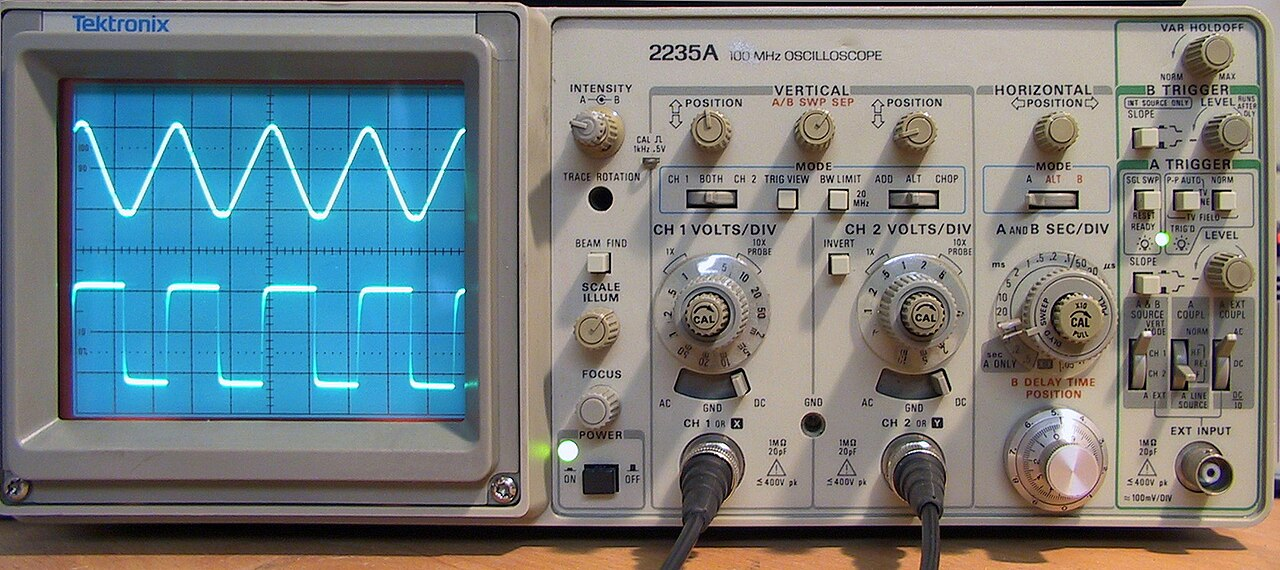
\includegraphics[width=0.60\linewidth]{images/book3/oscilloscope-sine-square.jpg}

{\small راسم اهتزاز يعرض جيبًا وموجة مربعة: فالجيب هو الإشارة التي يعيش عليها هذا الفصل، والموجة المربعة هي التي يفكّكها الفصل التالي إلى جيوب.}
\end{omfigure}

\section{النظام الجيبي الدائم}

\begin{proposition}[النظام الجيبي القسري]\label{prop:b1:sinusoidal-impedance:forced}
\index{نظام جيبي دائم}\index{نظام قسري}
في \omterm{def:b1:dc-circuits:linear}{دارة خطية} يقودها منبع جيبي تواتره الزاوي
$\omega$، يكون كل تيار وكل توتر، بعد أن تخبو الأنظمة العابرة،
جيبًا له \omterm{def:b1:wave-propagation:signal}{التواتر الزاوي} $\omega$ نفسه، ولكلٍّ سعته
وطوره: $x(t) = X\cos(\omega t + \varphi)$.
\end{proposition}

\begin{proof}
معادلات الدارة معادلات تفاضلية خطية ذات معاملات
ثابتة؛ وحلّها العام حلّ خاصّ زائد
حلول المعادلة المتجانسة، وهي عوابر
\cref{ch:b1:transient-regimes} وتتناقص (فلكل دارة حقيقية بعض
المقاومة). ويوجد حلّ خاصّ جيبي لأن
اشتقاق جيب تواتره $\omega$ يعطي جيبًا له
التواتر نفسه: فيمكن تحقيق المعادلات حدًّا حدًّا --- والطريقة
العقدية أدناه تبنيه صراحةً.
\end{proof}

\begin{definition}[السعة العقدية]\label{def:b1:sinusoidal-impedance:complex}
\index{سعة عقدية}\index{متجهة فرنل}
يُقرن بالجيب $x(t) = X\cos(\omega t + \varphi)$ الإشارةُ
العقدية $\underline{x}(t) = X\eu^{j(\omega t + \varphi)}$، بحيث
$x = \Rea(\underline{x})$، وتُقرن به \emph{السعة العقدية}
\[
\underline{X} = X\eu^{j\varphi}, \qquad \underline{x}(t) = \underline{X}\,\eu^{j\omega t},
\]
وهي تحمل السعة $X = \abs{\underline{X}}$ والطور
$\varphi = \arg\underline{X}$. ويرمز $j$ هنا إلى الوحدة التخيلية،
$j^2 = -1$، إذ حُفظ الحرف $i$ للتيارات. وإذا رُسمت
متجهةً طولها $X$ بالزاوية $\varphi$ كانت $\underline{X}$
\emph{متجهة فرنل}.
\end{definition}

\begin{proposition}[قواعد الطريقة العقدية]\label{prop:b1:sinusoidal-impedance:rules}
\begin{enumerate}
  \item العمليات الخطية تتبادل مع أخذ الجزء الحقيقي: \omterm{def:b1:sinusoidal-impedance:complex}{فالسعة
        العقدية} لمجموع هي مجموع السعات العقدية.
  \item الاشتقاق بالنسبة إلى الزمن يضرب \omterm{def:b1:sinusoidal-impedance:complex}{السعة
        العقدية} في $j\omega$؛ والمكاملة تقسمها على $j\omega$.
  \item قانونا كيرشوف، لكونهما خطيين، يصحّان من أجل السعات العقدية.
\end{enumerate}
\end{proposition}

\begin{proof}
$\Rea(\underline a + \underline b) = \Rea\underline a + \Rea\underline b$؛
و$\dd(\underline X\eu^{j\omega t})/\dd t = j\omega\underline X\eu^{j\omega t}$،
و$\dd x/\dd t = \Rea(\dd\underline x/\dd t)$ لأن الاشتقاق
خطي حقيقيًّا. ومجاميع التيارات عند عقدة والتوترات على امتداد
حلقة خطية.
\end{proof}

\begin{example}[جمع جيبين]\label{ex:b1:sinusoidal-impedance:add}
$3\cos\omega t + 4\sin\omega t$: السعتان العقديتان هما $3$ و
$4\eu^{-j\pi/2} = -4j$ (لأن $\sin\omega t = \cos(\omega t - \pi/2)$)؛
ومجموعهما $3 - 4j$ مقياسه $5$ وعمدته $-0.927\ \unit{rad}$:
أي $5\cos(\omega t - 0.927)$. ولا حاجة إلى أيّ متطابقة مثلثية.
\end{example}

\section{الممانعة}

\begin{definition}[الممانعة والمسايرة]\label{def:b1:sinusoidal-impedance:impedance}
\index{ممانعة}\index{مسايرة}\index{مفاعلة}
من أجل \omterm{def:b1:dc-circuits:linear}{ثنائي قطب خطي} في \omterm{prop:b1:sinusoidal-impedance:forced}{النظام الجيبي الدائم} (\omterm{thm:b1:dc-circuits:kirchhoff}{باصطلاح
المستقبِل})، تكون \emph{الممانعة} نسبةَ السعتين العقديتين
\[
\underline Z = \frac{\underline U}{\underline I} = Z\eu^{j\varphi}
\quad (\text{بالأوم}),
\]
ومقياسها $Z = U/I$ يربط السعتين، وعمدتها
$\varphi = \varphi_u - \varphi_i$ هي تقدّم طور التوتر على
التيار. ومقلوبها $\underline Y = 1/\underline Z$ هو
\emph{المسايرة} (بالسيمنس). والجزء الحقيقي من $\underline Z$ هو
مقاومتها، والجزء التخيلي \emph{مفاعلتها}.
\end{definition}

\begin{proposition}[ممانعات R و L و C]\label{prop:b1:sinusoidal-impedance:rlc}
\[
\underline Z_R = R, \qquad \underline Z_L = jL\omega, \qquad
\underline Z_C = \frac{1}{jC\omega} = -\frac{j}{C\omega} .
\]
\omterm{def:b1:dc-circuits:resistor}{الناقلة الأومية} تُبقي التوتر والتيار على الطور نفسه؛ وفي الوشيعة يتقدّم التوتر
على التيار بمقدار $\pi/2$؛ وفي المكثف يتأخر بمقدار $\pi/2$. وعند التواتر
المنخفض تؤول الوشيعة إلى سلك ويؤول المكثف إلى دارة مفتوحة؛ وعند
التواتر العالي يكون العكس.
\end{proposition}

\begin{proof}
$u = Ri$؛ و$u = L\,\dd i/\dd t \to \underline U = jL\omega\,\underline I$؛
و$i = C\,\dd u/\dd t \to \underline I = jC\omega\,\underline U$. و
عمدات $1$ و $j$ و $-j$ هي $0$ و $\pi/2$ و $-\pi/2$.
\end{proof}

\begin{proposition}[التجميع والمجزّئات والمبرهنات]\label{prop:b1:sinusoidal-impedance:assoc}
الممانعات على التسلسل تُجمع؛ والمسايرات على التفرع تُجمع؛ ومجزّئا التوتر
والتيار ومبرهنتا تيفنان ونورتن والتراكب و
مبرهنة ميلمان في \cref{ch:b1:dc-circuits} تصحّ كلها مع السعات
العقدية والممانعات بدلًا من التوترات والتيارات والمقاومات
الحقيقية.
\end{proposition}

\begin{proof}
كل برهان في \cref{ch:b1:dc-circuits} لم يستعمل إلا قانونَي كيرشوف و
خطية $u = Ri$، وكلاهما يصحّ في الصورة العقدية.
\end{proof}

\begin{example}[مجزّئ RC]\label{ex:b1:sinusoidal-impedance:rcdivider}
\omterm{def:b1:dc-circuits:resistor}{ناقلة أومية} $R$ ومكثف $C$ على التسلسل تحت $\underline E$، و
الخرج مأخوذ على طرفَي $C$: فيكون $\underline U_C = \underline E\,\dfrac{1/jC\omega}
{R + 1/jC\omega}$، أي $\dfrac{\underline E}{1 + jRC\omega}$. فالسعة
$E/\sqrt{1 + (RC\omega)^2}$، والطور $-\arctan(RC\omega)$: أي نفاذ
تامّ عند التواترات المنخفضة، و$1/\sqrt2$ و$-45^\circ$ عند
$\omega = 1/RC$، وهبوط بالمقدار $1/\omega$ بعدها --- أي مرشّح تمرير منخفض، وهو
موضوع \cref{ch:b1:filters-transfer-functions}.
\end{example}

\section{الدارة RLC على التسلسل: الرنين}

\begin{theorem}[رنين التيار]\label{thm:b1:sinusoidal-impedance:resonance}
\index{رنين}\index{رنين!التيار}\index{عرض النطاق}
\omterm{def:b1:dc-circuits:resistor}{ناقلة أومية} $R$ ووشيعة $L$ ومكثف $C$ على التسلسل تحت
$e(t) = E\cos\omega t$ تحمل تيارًا سعته العقدية
\[
\underline I = \frac{E}{R + j\left(L\omega - \dfrac{1}{C\omega}\right)},
\qquad
I = \frac{E}{\sqrt{R^2 + \left(L\omega - \dfrac{1}{C\omega}\right)^2}},
\qquad
\varphi_i = -\arctan\frac{L\omega - 1/C\omega}{R} .
\]
والسعة عظمى، $I_{\max} = E/R$، ويكون التيار والتوتر على الطور
نفسه، عند \emph{الرنين} $\omega_0 = 1/\sqrt{LC}$. ومع
$Q = L\omega_0/R = 1/(RC\omega_0)$ و $x = \omega/\omega_0$،
\[
\frac{I}{I_{\max}} = \frac{1}{\sqrt{1 + Q^2\left(x - \dfrac1x\right)^2}} ,
\]
ويكون \emph{\omterm{thm:b1:sinusoidal-impedance:resonance}{عرض النطاق}} --- أي مجال $\omega$ الذي يتحقق فيه
$I \geq I_{\max}/\sqrt2$ --- هو
\[
\Delta\omega = \omega_2 - \omega_1 = \frac{\omega_0}{Q} = \frac{R}{L} .
\]
\end{theorem}

\begin{proof}
الممانعات على التسلسل تُجمع: $\underline Z = R + jL\omega + 1/jC\omega$، و
$\underline I = \underline E/\underline Z$. والمقياس أكبر ما يكون حين
تنعدم \omterm{def:b1:sinusoidal-impedance:impedance}{المفاعلة} $L\omega - 1/C\omega$، أي عند $\omega_0$.
ونعامل $L\omega - 1/C\omega = L\omega_0(x - 1/x)$ ونقسم على $R$:
فيكون $L\omega_0/R = Q$. وعند حدَّي النطاق يكون $Q(x - 1/x) = \pm 1$، أي
$x^2 \mp x/Q - 1 = 0$، وجذراه الموجبان $x_{1,2} = \mp\frac{1}{2Q}
+ \sqrt{1 + \frac{1}{4Q^2}}$؛ والفرق بينهما $1/Q$.
\end{proof}

\begin{omfigure}
\begin{tikzpicture}
\begin{axis}[omaxis, width=7.6cm, height=5.4cm, xlabel={$\omega/\omega_0$}, ylabel={$I/I_{\max}$},
    xmin=0, xmax=2.1, ymin=0, ymax=1.45, xtick={0.5,1,1.5,2}, ytick={0.5,0.707,1},
    yticklabels={$0.5$,$\frac{1}{\sqrt2}$,$1$},
    legend style={at={(0.97,0.97)}, anchor=north east, font=\footnotesize, draw=none, fill=none}]
  \addplot[omProp, thick, domain=0.05:2.1, samples=300] {1/sqrt(1 + (1*(x - 1/x))^2)};
  \addlegendentry{$Q = 1$}
  \addplot[omDef, thick, domain=0.05:2.1, samples=300] {1/sqrt(1 + (3*(x - 1/x))^2)};
  \addlegendentry{$Q = 3$}
  \addplot[omThm, thick, domain=0.05:2.1, samples=500] {1/sqrt(1 + (10*(x - 1/x))^2)};
  \addlegendentry{$Q = 10$}
  \draw[dashed, omExo] (axis cs:0,0.707) -- (axis cs:2.1,0.707);
\end{axis}
\end{tikzpicture}\qquad
\begin{tikzpicture}
\begin{axis}[omaxis, width=7.0cm, height=5.4cm, xlabel={$\omega/\omega_0$}, ylabel={$\varphi_i$},
    xmin=0, xmax=2.1, ymin=-1.8, ymax=1.8, xtick={0.5,1,1.5,2}, ytick={-1.5708,0,1.5708},
    yticklabels={$-\frac{\pi}{2}$,$0$,$\frac{\pi}{2}$}]
  \addplot[omProp, thick, domain=0.05:2.1, samples=300] {-rad(atan(1*(x - 1/x)))};
  \addplot[omDef, thick, domain=0.05:2.1, samples=300] {-rad(atan(3*(x - 1/x)))};
  \addplot[omThm, thick, domain=0.05:2.1, samples=500] {-rad(atan(10*(x - 1/x)))};
\end{axis}
\end{tikzpicture}

{\small \omterm{prop:b1:transient-regimes:rlc}{الدارة RLC} على التسلسل: سعة التيار (يسارًا) وطوره
بالنسبة إلى المنبع (يمينًا) بدلالة $\omega/\omega_0$، من أجل
$Q = 1, 3, 10$. وتضيق الذروة كلما نما $Q$ ($\Delta\omega =
\omega_0/Q$)؛ ودون الرنين تكون الدارة سعوية (فيتقدّم
التيار)، وفوقه تحريضية (فيتأخر).}
\end{omfigure}

\begin{omfigure}
\begin{tikzpicture}[font=\small, x=1cm, y=1cm, >=Stealth]
  % phasors for RLC at omega above resonance: UR along I, UL +90, UC -90
  \draw[->, thick, omExo] (0,0) -- (2.6,0) node[right] {$\underline I$};
  \draw[->, very thick, omProp] (0,0) -- (1.6,0) node[midway, below] {$\underline U_R = R\underline I$};
  \draw[->, very thick, omDef] (1.6,0) -- (1.6,2.4) node[left, pos=0.8] {$\underline U_L = jL\omega\underline I$};
  \draw[->, very thick, omDef!60] (1.78,2.4) -- (1.78,1.1) node[right, midway] {$\underline U_C = \underline I/jC\omega$};
  \draw[->, very thick, omThm] (0,0) -- (1.6,1.1) node[midway, above left, xshift=-1pt] {$\underline E$};
  \draw (0.6,0) arc (0:34.5:0.6); \node at (0.85,0.2) {$\varphi$};
\end{tikzpicture}

{\small مخطط متجهات فرنل \omterm{prop:b1:transient-regimes:rlc}{للدارة RLC} على التسلسل فوق الرنين: $\underline U_R$
على امتداد $\underline I$، و$\underline U_L$ متقدمةً ربع دورة، و$\underline U_C$
متأخرةً ربع دورة؛ ومجموعها $\underline E$ يتقدّم على التيار بمقدار
$\varphi$. وعند الرنين تتلاشى $\underline U_L$ و $\underline U_C$ ويكون
$\underline E = \underline U_R$.}
\end{omfigure}

\begin{proposition}[تضخيم التوتر]\label{prop:b1:sinusoidal-impedance:overvoltage}
\index{رنين!التوتر}\index{فرط التوتر}
عند الرنين يكون للتوترين بين طرفَي الوشيعة والمكثف
السعة $QE$ نفسها وطوران متعاكسان: فمن أجل $Q \gg 1$ يحمل المكثف
توترًا أكبر $Q$ مرة من توتر المنبع. والسعة
$U_C(\omega)$ نفسها تبلغ ذروة، من أجل $Q > 1/\sqrt2$، عند $\omega_r =
\omega_0\sqrt{1 - 1/2Q^2}$، دون $\omega_0$ بقليل، حيث
$U_{C,\max} = QE/\sqrt{1 - 1/4Q^2}$.
\end{proposition}

\begin{proof}
عند $\omega_0$ يكون $\underline U_C = \underline I/jC\omega_0 = -jQE$ و
$\underline U_L = jL\omega_0\underline I = jQE$ لأن $I = E/R$. وفي
الحالة العامة $U_C = I/C\omega = E/\sqrt{(1 - x^2)^2 + x^2/Q^2}$ (بضرب
البسط والمقام في $1/C\omega_0$)؛ ومربع المقام
هو $(1 - x^2)^2 + x^2/Q^2$، وهو ثلاثي حدود في $x^2$ يصغر عند $x^2 =
1 - 1/2Q^2$ حين يكون ذلك موجبًا، وأصغره $1/Q^2 - 1/4Q^4$.
\end{proof}

\begin{example}[ضبط مذياع]\label{ex:b1:sinusoidal-impedance:radio}
وشيعة $L = \qty{200}{\micro H}$ ومكثف متغير: فالسعة $C =
\qty{127}{pF}$ تضبط $f_0 = \qty{1.00}{MHz}$. ومع مقاومة سلك الوشيعة
$R = \qty{12.6}{\ohm}$ يكون $L\omega_0 = \qty{1257}{\ohm}$ و
$Q = 100$: \omterm{thm:b1:sinusoidal-impedance:resonance}{فعرض النطاق} $\Delta f = f_0/Q = \qty{10}{kHz}$ --- وهو عرض
قناة إذاعية --- ويصير التوتر \qty{10}{\micro V} الذي يحرّضه مرسِل بعيد
مقدارًا قدره $QE = \qty{1}{mV}$ على طرفَي المكثف، بلا مقابل.
وتبني مسألة نهاية الأسبوع هذا المستقبِل.
\end{example}

\begin{remark}[لماذا $Q$ من جديد]\label{rem:b1:sinusoidal-impedance:Q}
\omterm{def:b1:transient-regimes:secondorder}{عامل الجودة} $Q$ في هذا الفصل هو $Q$ في \cref{ch:b1:transient-regimes}:
فالدارة التي ترنّ نحو $Q$ تذبذبة عند قرعها هي
التي ترنّ على نطاق عرضه $\omega_0/Q$ عند قيادتها. وكلاهما
يعبّر عن نسبة واحدة: $2\pi$ مضروبًا في الطاقة المخزونة على الطاقة
المتبددة في كل دور (\cref{exo:b1:sinusoidal-impedance:12}). و
الرنين الحادّ والرنين الطويل خاصية واحدة، وكذلك
الاستجابة البطيئة: فمرشّح عرض نطاقه $\Delta\omega$ يحتاج إلى زمن من
رتبة $1/\Delta\omega$ ليستقرّ.
\end{remark}

\section{الاستطاعة في النظام الجيبي}

\begin{definition}[القيمة الفعّالة]\label{def:b1:sinusoidal-impedance:rms}
\index{قيمة جذر متوسط المربعات}\index{قيمة فعّالة}
\emph{جذر متوسط المربعات} (أو القيمة الفعّالة) لإشارة
دورية $x(t)$ هو $X_{\mathrm{rms}} = \sqrt{\langle x^2\rangle}$، أي
الجذر التربيعي لمتوسط $x^2$ الزمني على دور. ومن أجل جيب
سعته $X$ يكون $X_{\mathrm{rms}} = X/\sqrt2$. والقيمة \qty{230}{V} للتيار
المنزلي قيمة فعّالة؛ وسعته \qty{325}{V}.
\end{definition}

\begin{theorem}[الاستطاعة المتوسطة]\label{thm:b1:sinusoidal-impedance:power}
\index{استطاعة متوسطة}\index{عامل الاستطاعة}\index{استطاعة تفاعلية}
ثنائي قطب فيه $u = U\cos\omega t$ و $i = I\cos(\omega t - \varphi)$
(\omterm{thm:b1:dc-circuits:kirchhoff}{باصطلاح المستقبِل}) يتلقى الاستطاعة اللحظية $p = ui$، ومتوسطها
\[
P = \tfrac12\,UI\cos\varphi = U_{\mathrm{rms}}I_{\mathrm{rms}}\cos\varphi
= \tfrac12\Rea\!\big(\underline U\,\underline I^{\,*}\big) = \tfrac12\Rea(\underline Z)\,I^2,
\]
حيث $\cos\varphi$ هو \emph{\omterm{thm:b1:sinusoidal-impedance:power}{عامل الاستطاعة}}. \omterm{def:b1:dc-circuits:resistor}{والناقلة الأومية} تتلقى
$\tfrac12 RI^2 = RI_{\mathrm{rms}}^2$؛ أما الوشيعة أو المكثف المثالي
($\varphi = \pm\pi/2$) فلا يتلقى \omterm{thm:b1:sinusoidal-impedance:power}{استطاعة متوسطة} --- إذ يخزّن الطاقة
نصف دور ويعيدها في النصف الآخر.
\end{theorem}

\begin{proof}
$p = UI\cos\omega t\cos(\omega t - \varphi) = \tfrac12 UI[\cos\varphi +
\cos(2\omega t - \varphi)]$؛ ومتوسط الحدّ الثاني معدوم. ومع
$\underline U = U$ و $\underline I = I\eu^{-j\varphi}$ يكون
$\underline U\,\underline I^* = UI\eu^{j\varphi}$، وجزؤه الحقيقي
$UI\cos\varphi$؛ و$\underline U = \underline Z\,\underline I$ يعطي
$\underline U\,\underline I^* = \underline Z I^2$.
\end{proof}

\begin{omfigure}
\begin{tikzpicture}
\begin{axis}[omaxis, axis x line=bottom, width=11.5cm, height=5cm, xlabel={$t/T$}, ylabel={$p$},
    xmin=0, xmax=2, ymin=-0.5, ymax=1.15, xtick={0.5,1,1.5,2}, ytick={0,0.5,1},
    yticklabels={$0$,$P$,$UI$}]
  \addplot[omDef, thick, domain=0:2, samples=300] {cos(deg(2*pi*x))*cos(deg(2*pi*x) - 60)};
  \addplot[omThm, thick, dashed, domain=0:2, samples=2] {0.25};
  \addplot[omExo, dashed, domain=0:2, samples=2] {0};
  \node[omDef, font=\footnotesize] at (axis cs:1.62,0.95) {$p(t) = ui$, $\varphi = 60^\circ$};
  \node[omThm, font=\footnotesize] at (axis cs:0.5,0.95) {المتوسط $P = \tfrac12 UI\cos\varphi$ (المتقطع)};
\end{axis}
\end{tikzpicture}

{\small الاستطاعة اللحظية التي يتلقاها ثنائي قطب بفرق طور قدره $60^\circ$
بين التيار والتوتر: فهي تنبض عند $2\omega$، وتغوص دون الصفر
(أي طاقة تعود إلى المنبع)، ومتوسطها $\tfrac12 UI\cos\varphi$
--- أي نصف ما كانت ستكونه لو كانا على الطور نفسه.}
\end{omfigure}

\begin{example}[تصحيح عامل الاستطاعة]\label{ex:b1:sinusoidal-impedance:pf}
محرك ورشة على \qty{230}{V} فعّالة يسحب \qty{2.0}{kW} مع
$\cos\varphi = 0.70$ (تحريضي): فيكون $I_{\mathrm{rms}} = 2000/(230 \times
0.70) = \qty{12.4}{A}$، في مقابل \qty{8.7}{A} لو كان \omterm{thm:b1:sinusoidal-impedance:power}{عامل الاستطاعة}
$1$ --- والتيار الزائد يسخّن كبلات الشركة بلا فائدة، ومن هنا
الغرامة. ومكثف على التفرع يوفّر محليًّا تأرجحات طاقة الوشيعة كل ربع
دور: أي إن \emph{\omterm{thm:b1:sinusoidal-impedance:power}{الاستطاعة التفاعلية}} $P\tan\varphi =
\qty{2.0}{kvar}$ تحتاج إلى $C = P\tan\varphi/(\omega U_{\mathrm{rms}}^2)
\approx \qty{120}{\micro F}$ عند \qty{50}{Hz}، فيهبط تيار الخط
إلى \qty{8.7}{A}.
\end{example}

\section{تمارين}

\begin{exercise}[$\star$]\label{exo:b1:sinusoidal-impedance:1}
أعطِ \omterm{def:b1:sinusoidal-impedance:complex}{السعة العقدية} للتوتر $u = 5\cos(\omega t + \pi/3)$ (بالفولط)، بالصورتين
القطبية والديكارتية. وباستعمال السعات العقدية، اكتب $3\cos\omega t
+ 4\sin\omega t$ جيبَ تمام واحدًا.
\end{exercise}

\begin{exercise}[$\star$]\label{exo:b1:sinusoidal-impedance:2}
احسب \omterm{def:b1:sinusoidal-impedance:impedance}{ممانعة} $R = \qty{100}{\ohm}$ و $L = \qty{0.10}{H}$ و
$C = \qty{10}{\micro F}$ عند \qty{50}{Hz} وعند \qty{1.0}{kHz}. وأعطِ
مقياس وطور \omterm{def:b1:sinusoidal-impedance:impedance}{ممانعة} $R$ و $L$ على التسلسل عند
\qty{50}{Hz}.
\end{exercise}

\begin{exercise}[$\star$]\label{exo:b1:sinusoidal-impedance:3}
التيار المنزلي \qty{230}{V} فعّالة: فما سعته؟ ومدفأة \qty{2.0}{kW}:
التيار الفعّال والأعظمي. وبيّن أن \omterm{thm:b1:sinusoidal-impedance:power}{الاستطاعة المتوسطة} في \omterm{def:b1:dc-circuits:resistor}{ناقلة أومية}
هي $RI_{\mathrm{rms}}^2$.
\end{exercise}

\begin{exercise}[$\star$]\label{exo:b1:sinusoidal-impedance:4}
\omterm{prop:b1:transient-regimes:rlc}{دارة RLC} على التسلسل: $L = \qty{10}{mH}$ و $C = \qty{100}{nF}$ و $R = \qty{100}{\ohm}$
و $E = \qty{1.0}{V}$. أعطِ $f_0$ و $Q$ \omterm{thm:b1:sinusoidal-impedance:resonance}{وعرض النطاق} بالهرتز و
سعة التيار عند الرنين.
\end{exercise}

\begin{exercise}[$\star\star$]\label{exo:b1:sinusoidal-impedance:5}
مجزّئ RC، والخرج على طرفَي $C$: $R = \qty{1.0}{k\ohm}$ و $C = \qty{159}{nF}$.
عند أيّ تواتر يكون الخرج $1/\sqrt2$ من الدخل؟ وأعطِ
نسبة سعة الخرج وطوره عند \qty{1.0}{kHz} وعند \qty{10}{kHz}.
\end{exercise}

\begin{exercise}[$\star\star$]\label{exo:b1:sinusoidal-impedance:6}
عند تواتر ما تكون \omterm{prop:b1:transient-regimes:rlc}{لدارة RLC} على التسلسل $R = \qty{100}{\ohm}$ و $L\omega =
\qty{250}{\ohm}$ و $1/C\omega = \qty{100}{\ohm}$، مع $E = \qty{1.0}{V}$.
احسب $\underline Z$ وسعة التيار وطوره والتوترات
الثلاثة؛ وارسم مخطط متجهات فرنل. وهل الدارة فوق الرنين أم
دونه؟
\end{exercise}

\begin{exercise}[$\star\star$]\label{exo:b1:sinusoidal-impedance:7}
مذياع: $L = \qty{200}{\micro H}$ و $C$ قابلة للضبط من \qty{50}{} إلى
\qty{500}{pF}. أوجد مجال التواترات، والسعة الموافقة للتواتر
\qty{1.00}{MHz}، ثم، مع $Q = 100$، \omterm{thm:b1:sinusoidal-impedance:resonance}{عرض النطاق} والتوهين
(أي نسبة السعات) لمحطة تبعد \qty{9}{kHz}. ومع قوة محركة هوائية قدرها
\qty{10}{\micro V}: ما التوتر على طرفَي $C$ عند الرنين؟
\end{exercise}

\begin{exercise}[$\star\star$]\label{exo:b1:sinusoidal-impedance:8}
اشتقّ تواترَي نصف الاستطاعة \omterm{prop:b1:transient-regimes:rlc}{للدارة RLC} على التسلسل وبيّن أن
فرقهما $\omega_0/Q$ وجداءهما $\omega_0^2$.
\end{exercise}

\begin{exercise}[$\star\star$]\label{exo:b1:sinusoidal-impedance:9}
محرك على \qty{230}{V} فعّالة عند \qty{50}{Hz} يمتصّ \qty{2.0}{kW} مع
$\cos\varphi = 0.70$. احسب التيار الفعّال \omterm{thm:b1:sinusoidal-impedance:power}{والاستطاعة التفاعلية} و
السعة الموضوعة على التفرع التي ترفع \omterm{thm:b1:sinusoidal-impedance:power}{عامل الاستطاعة} إلى $1$، والتيار
الجديد. وخط التغذية مقاومته \qty{0.50}{\ohm}: فما ضياعات جول قبل
ذلك وبعده؟
\end{exercise}

\begin{exercise}[$\star\star\star$]\label{exo:b1:sinusoidal-impedance:10}
\omterm{prop:b1:transient-regimes:rlc}{دارة RLC} على التفرع يغذّيها \omterm{def:b1:dc-circuits:sources}{منبع تيار}: اكتب \omterm{def:b1:sinusoidal-impedance:impedance}{المسايرة}، وبيّن أن
التوتر أعظمي عند $\omega_0 = 1/\sqrt{LC}$ ويساوي $RI$
هناك، وأن \omterm{thm:b1:sinusoidal-impedance:resonance}{عرض النطاق} $\Delta\omega = 1/RC$، أي $Q =
R\sqrt{C/L}$. والأعداد: $R = \qty{10}{k\ohm}$ و $L = \qty{1.0}{mH}$ و
$C = \qty{1.0}{nF}$.
\end{exercise}

\begin{exercise}[$\star\star\star$]\label{exo:b1:sinusoidal-impedance:11}
بيّن أن توتر مكثف \omterm{prop:b1:transient-regimes:rlc}{دارة RLC} على التسلسل هو $U_C = E/\sqrt{(1 -
x^2)^2 + x^2/Q^2}$، وأنه يبلغ ذروته عند $x_r = \sqrt{1 - 1/2Q^2}$ إذا كان
$Q > 1/\sqrt2$، واحسب $x_r$ و $U_{C,\max}/E$ من أجل $Q = 3.16$.
وماذا يحدث من أجل $Q < 1/\sqrt2$؟
\end{exercise}

\begin{exercise}[$\star\star\star$]\label{exo:b1:sinusoidal-impedance:12}
عند رنين \omterm{prop:b1:transient-regimes:rlc}{دارة RLC} على التسلسل، بيّن أن الطاقة المخزونة الكلية
$\tfrac12 Li^2 + \tfrac12 Cu_C^2$ ثابتة وتساوي $\tfrac12 LI^2$،
واحسب الطاقة المتبددة في $R$ في كل دور، وبرهن على أن
$2\pi\,(\text{المخزونة})/(\text{المتبددة في كل دور}) = Q$.
\end{exercise}

\begin{omfigure}

\includegraphics[width=0.55\linewidth]{images/book3/ai/b3-08-vintage-radio-tuning.png}

{\small ضبط مذياع صمّامي: إدارة المقبض تغيّر مكثفًا، والمكثف يثبّت تواتر رنين دارة $LC$، فتكون المحطة التي يوافق تواترها هي المسموعة --- وهي مسألة نهاية الأسبوع.}
\end{omfigure}

\section{مسألة: مستقبِل المذياع الرنّان}

\begin{problem}[{مسألة نهاية الأسبوع --- وشيعة ومكثف متغير و
هوائي: كيف يلتقط رنينٌ متسلسل محطة واحدة من مئة،
ويضرب إشارتها الخافتة في مئة، ولماذا لا يمكن جعله
انتقائيًّا بلا حدّ}]
\label{pb:b1:sinusoidal-impedance:1}
يُنمذج الهوائي بقوة محركة جيبية مثالية $e(t) = E\cos\omega t$
على التسلسل مع وشيعة $L = \qty{200}{\micro H}$ مقاومة سلكها
$R = \qty{12.6}{\ohm}$، ومكثف متغير $C$. ويقرأ
المستقبِل التوتر على طرفَي $C$. وفي ما بعد (الجزء IV) تُؤخذ مقاومة الهوائي
نفسه $R_a = \qty{50}{\ohm}$ في الحسبان.

\medskip
\noindent\textbf{الجزء I --- التيار الرنّان.}
\begin{enumerate}
  \item اكتب \omterm{def:b1:sinusoidal-impedance:impedance}{الممانعة} العقدية للدارة المتسلسلة.
  \item أعطِ \omterm{def:b1:sinusoidal-impedance:complex}{السعة العقدية} للتيار، ثم سعته
        $I(\omega)$ وطوره $\varphi_i(\omega)$ بالنسبة إلى $e$.
  \item بيّن أن $I$ أعظمي عند $\omega_0 = 1/\sqrt{LC}$؛ وأعطِ
        $I_{\max}$ والطور عندئذٍ.
  \item أيّ سعة تضبط $f_0 = \qty{1.000}{MHz}$؟ واحسب
        $L\omega_0$.
  \item عرّف $Q = L\omega_0/R$ واحسبه.
  \item بيّن أن $I/I_{\max} = 1/\sqrt{1 + Q^2(x - 1/x)^2}$ مع
        $x = \omega/\omega_0$.
  \item اذكر إشارة $\varphi_i$ دون الرنين وفوقه ثم
        فسّرها (سلوك سعوي أم تحريضي).
\end{enumerate}

\medskip
\noindent\textbf{الجزء II --- الانتقائية.}
\begin{enumerate}[resume]
  \item اكتب الشرط الذي يعرّف التواترين اللذين يكون عندهما
        $I = I_{\max}/\sqrt2$.
  \item حلّه وبيّن أن $\Delta\omega = \omega_2 - \omega_1 =
        \omega_0/Q$.
  \item احسب \omterm{thm:b1:sinusoidal-impedance:resonance}{عرض النطاق} $\Delta f$ لهذا المستقبِل.
  \item محطة ثانية تبثّ عند \qty{1.010}{MHz}، وثالثة عند
        \qty{1.020}{MHz}: احسب نسبة السعات $I/I_{\max}$ لكلٍّ
        منهما، ونسبة الاستطاعات الموافقة بالديسيبل.
  \item تتباعد المحطات الإذاعية \qty{9}{} إلى \qty{10}{kHz}. فهل
        المستقبِل انتقائي بما فيه الكفاية؟ وما الذي يحسّنه؟
  \item يمكن ضبط المكثف بين \qty{50}{} و\qty{500}{pF}:
        فأيّ نطاق تواتري يغطّيه المستقبِل؟
\end{enumerate}

\medskip
\noindent\textbf{الجزء III --- تضخيم التوتر.}
\begin{enumerate}[resume]
  \item عبّر عن \omterm{def:b1:sinusoidal-impedance:complex}{السعة العقدية} لتوتر المكثف وبيّن
        أن سعته عند الرنين هي $QE$.
  \item القوة المحركة للهوائي $E = \qty{10}{\micro V}$: احسب $I_{\max}$
        وتوتر المكثف عند الرنين. علّق على ذلك.
  \item بيّن أن لتوتر الوشيعة السعة نفسها وأنه في
        تعاكس طور مع توتر المكثف عند الرنين: فماذا
        ``يرى'' المنبع؟
  \item احسب الطاقة المخزونة في الدارة عند الرنين و
        الطاقة المتبددة في كل دور؛ وتحقق من أن نسبتهما مضروبةً في
        $2\pi$ تساوي $Q$.
  \item انطلاقًا من \cref{ch:b1:transient-regimes}، ما \omterm{def:b1:transient-regimes:firstorder}{ثابت الزمن}
        $\tau = 2Q/\omega_0$ لهذه الدارة؟ ولماذا يشوّه $Q$ العالي جدًّا
        الكلام والموسيقى في النهاية (وعرض نطاق الصوت
        نحو \qty{5}{kHz} في الإذاعة)؟
  \item لو تضاعفت مقاومة سلك الوشيعة (بسلك أرقّ)، فكيف تتغير
        $Q$ \omterm{thm:b1:sinusoidal-impedance:resonance}{وعرض النطاق} وتوتر المكثف؟
\end{enumerate}

\medskip
\noindent\textbf{الجزء IV --- مقاومة الهوائي والاستطاعة.}
\begin{enumerate}[resume]
  \item مع $R_a = \qty{50}{\ohm}$ على التسلسل، أعد حساب $Q$ و
        \omterm{thm:b1:sinusoidal-impedance:resonance}{عرض النطاق} وتوتر المكثف من أجل $E = \qty{10}{\micro V}$.
        واستنتج.
  \item احسب \omterm{thm:b1:sinusoidal-impedance:power}{الاستطاعة المتوسطة} التي تقدّمها القوة المحركة للهوائي عند
        الرنين والكسر المتبدد في $R_a$.
  \item تطلب مبرهنة الاستطاعة العظمى مقاومة حمولة تساوي
        $R_a$: فلماذا يتعارض هذا الهدف مع الانتقائية؟
  \item تصل المستقبِلات الحقيقية الهوائي بمأخذ على الوشيعة، أو
        عبر مكثف اقتران صغير. فسّر نوعيًّا ما الذي
        يحققه ذلك.
  \item باستعمال $P = \tfrac12 UI\cos\varphi$، احسب \omterm{thm:b1:sinusoidal-impedance:power}{عامل الاستطاعة} عند
        تواترَي نصف الاستطاعة وفسّر الاسم
        ``نصف الاستطاعة''.
  \item لخّص التصميم: ماذا يشتري $Q$، وماذا يكلّف، وما
        القيمة المختارة لمستقبِل عند \qty{1}{MHz} بقنوات عرضها
        \qty{10}{kHz}.
\end{enumerate}
\end{problem}
